\documentclass[tikz,border=2mm]{standalone}
\usetikzlibrary{positioning,calc}

\tikzset{
  redondo/.style={draw=blue,line width=1pt,rounded corners=3pt,text width=#1},
  punto/.style={fill=red,circle,inner sep=1.25pt},
  tresp/.pic={
    \node[punto] at (0.25,0) {};
    \node[punto] at (0.5,0) {};
    \node[punto] at (0.75,0) {};
  },
  dosp/.pic={
    \node[punto] at (0.25,0) {};
    \node[punto] at (0.5,0) {};
  },
  cuadra/.style={fill=teal,minimum size=10pt},
  arr/.style={line width=1pt,draw=green!70!black,->,>=latex}  
}

\begin{document}

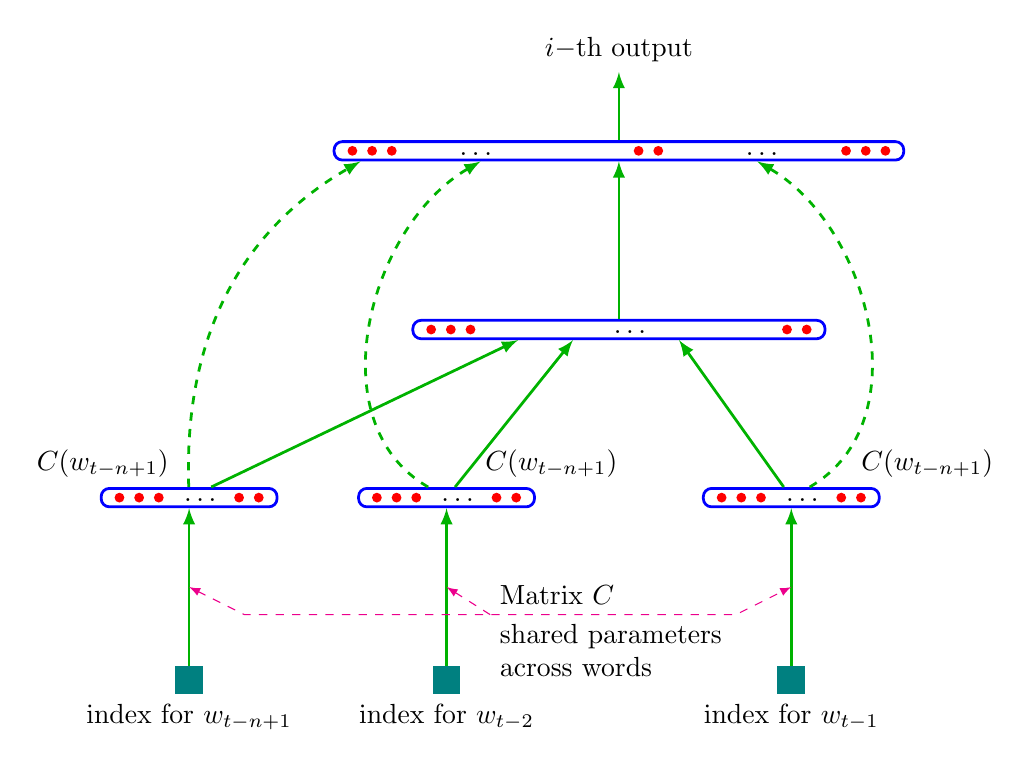
\begin{tikzpicture}[node distance=2cm and 1cm]
	\node[redondo=7cm](upper){};
	\pic at (upper.west) {tresp};
	\pic at (upper.center) {dosp};
	\pic at ([xshift=-1cm]upper.east) {tresp};
	\node[] at ([yshift=-1pt]$ (upper.center)!0.5!(upper.west) $ ) {$\ldots$};
	\node[] at ([yshift=-1pt]$ (upper.center)!0.5!(upper.east) $ ) {$\ldots$};

	\node[redondo=5cm,below=of upper] (middle) {};
	\pic at (middle.west) {tresp};
	\pic at ([xshift=-0.75cm]middle.east) {dosp};
	\node[] at ([xshift=4pt,yshift=-1pt]middle) {$\ldots$};

	\node[redondo=2cm,below=of middle,anchor=east,xshift=-30pt,label={20:$C(w_{t-n+1})$}] (lowermiddle) {};
	\node[redondo=2cm,below=of middle,anchor=west,xshift=30pt,label={10:$C(w_{t-n+1})$}] (lowerright) {};
	\node[redondo=2cm,left=of lowermiddle,label={above left:$C(w_{t-n+1})$}] (lowerleft) {};

	\foreach \Valor/\NodeLabel in {left/n+1,middle/2,right/1/} {
  		\pic at (lower\Valor.west) {tresp};
  		\pic at ([xshift=-0.75cm]lower\Valor.east) {dosp};
  		\node[cuadra,below=of lower\Valor,label={below:{index for $w_{t-\NodeLabel}$}}] (cuadra\Valor) {};
  		\node[] at ([xshift=4pt,yshift=-1pt]lower\Valor) {$\ldots$};
	}

	\draw[arr,dashed] (lowerleft) to[out=92,in=210] ([xshift=10pt]upper.south west);
	\draw[arr,dashed] (lowermiddle) to[out=150,in=210] ([xshift=-50pt]upper.south);
	\draw[arr,dashed] (lowerright) to[out=30,in=-30] ([xshift=50pt]upper.south);
	\foreach \Valor in {left,middle,right} {
    		\draw[arr] (cuadra\Valor) -- coordinate (aux\Valor) (lower\Valor);
    	}
	\foreach \Valor/\Angulo in {left/186,middle/193,right/350} {
    		\draw[arr] (lower\Valor) -- (middle.\Angulo);
	}
	
	\draw[arr] (middle) -- (upper);
	\draw[arr] (upper) -- ++(0pt,1cm) node[above] {$i-$th output};
	\draw[<->,magenta,dashed,>=latex] (auxleft) -- ++(20pt,-10pt) -- ([shift={(-20pt,-10pt)}]auxright) coordinate[pos=0.5] (auxc) -- (auxright);
	\draw[->,magenta,dashed,>=latex] (auxc) -- (auxmiddle);
	\node[anchor=south west] at (auxc) {Matrix $C$};    
	\node[anchor=north west,align=left] at (auxc) {shared parameters \\ across words};    
\end{tikzpicture}

\end{document}